%!TEX root = main.tex
\section{Contenidos del paquete KSource}

La herramienta KSource cuenta con los siguiente componentes principales:
\begin{itemize}
	\item Biblioteca en Python, para estimación de densidad. Aquí se encuentras las herramientas necesarias para crear y optimizar una fuente KSource en base a una lista de partículas. Se puede además analizar su estadística, generar gráficos de las distribuciones, y exportar la fuente creada.
	\item Biblioteca en C, para muestreo. Aquí se encuentras las herramientas necesarias para muestrear nuevas partículas, en base a una fuente KSource previamente creada.
	\item Aplicación de línea de comando. Permite ejecutar un re-muestreo de partículas, en base a una fuente KSource previamente creada, obteniéndose una lista de partículas de longitud arbitraria. También permite acceder de forma simple a un conjunto de plantillas para las operaciones usuales con KSource.
\end{itemize}


\section{El formato de fuente KSource}

Descripción de la estructura con la que se representa una fuente KSource:
\begin{itemize}
	\item Listas de partículas MCPL
	\item Geometría
	\item Anchos de banda
	\item Archivo de parámetros XML
\end{itemize}

La herramienta KSource cuenta con librerías para modelar fuentes distribucionales de partículas en Python y C. En ambos casos se define la estructura \verb|KSource|, la cual a su vez posee dos subestructuras: \verb|PList| y \verb|Geometry|. Éstas modelan los dos componentes fundamentales de una fuente KSource: La lista de partículas y su geometría.

\subsection{Listas de partículas}

Las listas de partículas utilizadas en KSource utilizan el formato MCPL [CITA???]. El mismo permite la comunicación con los siguientes códigos Monte Carlo:
\begin{itemize}
	\item MCNP (version??)
	\item PHITS
	\item McStas
	\item GEANT4
	\item TRIPOLI-4
\end{itemize}
Esto quiere decir que es posible convertir las listas de partículas registradas por cualquiera de estos códigos a MCPL, y viceversa. El \emph{software} asociado al formato MCPL está incluido en la distribución de KSource, incluyendo funcionalidades extra, como la posibilidad de comunicación con TRIPOLI-4.

La estructura \verb|PList| empleada en las librerías administra la comunicación con el archivo MCPL. Además de la lectura y escritura, se incluye la posibilidad de aplicar una traslación y rotación a las partículas inmediatamente despues de leerlas, lo cual puede ser útil al conectar simulación con distinto sistema de referencia.

\subsection{Geometría}

A pesar de su nombre, la estructura \verb|Geometry| no sólo administra la geometría de fuente, sino la manera en que se debe tratar la energía y dirección de las partículas. El objetivo fundamental de esta estructura es convertir el conjunto de parámetros que definen una partícula, es decir energía, posición y dirección, a un vector sobre el que pueda suponerse una métrica euclidiana. Dicho vector es el que se utilizará como $x$ en las expresiones de la Subsección \ref{subsec:kde}.

Para dar versatilidad al tratamiento energético, espacial y angular deseado, la estructura \verb|Geometry| posee a su vez un conjunto de subestructuras de tipo \verb|Metric|. Usualmente se cuenta con tres de éstas: una para la energía, una para la posición, y una para la dirección. Cada \verb|Metric| define la métrica con la que se tratará cada conjunto de variables. Los objetos \verb|Metric| pueden elegirse del conjunto de métricas implementadas:
\begin{itemize}
	\item \verb|Energy|: tratamiento simple de la energía, sin transformaciones.
	\item \verb|Lethargy|: emplear letargía en lugar de energía.
	\item \verb|Vol|: tratamiento espacial volumétrico.
	\item \verb|SurfXY|: tratamiento espacial plano en XY.
	\item \verb|Guide|: geometría de guía de sección rectangular, con tratamiento de los ángulos basado en la superficie de cada espejo.
	\item \verb|Polar|: tratamiento de la dirección en base a los ángulo $\theta$ (distancia a la dirección $\hat{z}$) y $\phi$ (acimut medido desde la dirección $\hat{x}$).
	\item \verb|PolarMu|: igual a \verb|Polar|, pero con $\mu = cos(\theta)$ en lugar de $\theta$.
	\item \verb|Isotrop|: tratamiento simple de la dirección, basado en el versor unitario de dirección.
\end{itemize}

En la biblioteca de Python, la función principal tanto de \verb|Geometry| como de \verb|Metric| es la de transformar las partículas en el formato de partícula de MCPL a un vector de \verb|numpy|, lo cual se logra a través de las funciones \verb|transform| e \verb|inverse_transform|.

En la biblioteca de C, por su parte, la función principal de \verb|Geometry| y \verb|Metric| es la de perturbar partículas, respetando la métrica correspondiente y con los anchos de banda provistos. Esto se logra con las funciones \verb|[MetricName]_perturb|, donde \verb|[MetricName]| se debe reemplazar por el nombre de cada métrica.

\subsection{Archivos de parámetros XML}

Las fuentes creadas en Python, luego de la optimización, pueden guardarse en un archivo de parámetros en formato XML. En el mismo se registran los parámetros que definen las estructuras \verb|PList| y \verb|Geometry| que componen la fuente \verb|KSource|, así como el \emph{path} al archivo MCPL a utilizar. Este archivo de parámetros puede luego utilizarse para reconstruir la fuente mediante la biblioteca en C, o bien para re-muestrear directamente mediante la aplicación de línea de comando.


\section{Flujo de trabajo}

El esquema del flujo de trabajo típico con la herramienta KSource se esquematiza en la Figura \ref{fig:flujo}. Se parte de una lista de partículas inicial, la cual puede, o no, haber sido creada en una simulación anterior, y luego se ejecuta cierto número de simulaciones Monte Carlo. Cada una de ellas emplea una fuente de partículas KSource basada en la lista de partículas registrada inmediatamente antes, y registra una nueva lista de partículas para la etapa siguiente. Dependiendo del problema, pueden obtenerse resultados útiles en todas las simulaciones (por ejemplo, al construir un mapa de dosis), o bien sólo en la última (por ejemplo, al calcular el flujo en un punto de interés). Cada simulación cubre una región de la geometría modelada progresivamente más lejana a la fuente inicial, alcanzando distancias que no serían alcanzables en una sola corrida.

\begin{figure}[htbp!]
	\centering
	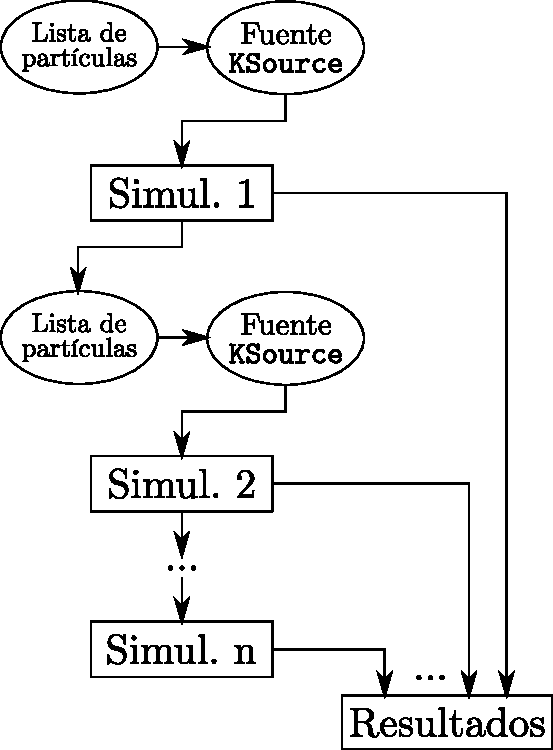
\includegraphics[width=.7\textwidth]{figs/flujo_trabajo.pdf}
	\caption{Esquema del flujo de trabajo típico.}
	\label{fig:flujo}
\end{figure}

Cada construcción de una fuente KSource en base a una lista de partículas se realiza mediante la API en Python, y culmina al exportar un archivo de parámetros XML. Se provee una plantilla con el código requerido para dicha tarea en el archivo \verb|preproc_tracks.ipynb|.

\subsection{Acople entre óptica neutrónica y transporte con McStas}

\subsection{Fuentes de activación con TRIPOLI-4}